\chapter{Overview}
\section{Introduction}
In typical undergraduate courses in theoretical computer science, a major aspect is to discuss different models of computability and
their expressiveness. One important result is, that primitive recursion is not Turing complete, i.e. not equivalent to Turing machines or $\mu$-recursion.
In \cite{Hoffmann2018}, the difference in computational power between $\mu$-recursion and primitive-recursive computation is presented by
the languages WHILE and LOOP, where WHILE is a Turing-complete imperative language
that offers basic control constructs like while loops and if-then-else, and LOOP is a restriction of WHILE that allows only a restricted 
loop construct \textit{\textbf{loop} x \textbf{do} ... \textbf{enddo}}, which is to be understood as "execute ... as often as the value of x".

In preliminary work, an interpreter for a variation of this two languages was developed \cite{Gebhard2018}. Currently the only available IDE for
this languages is IntelliJ in combination with a plugin that is released together with the interpreter. The goal of this project was
to develop an web-based interactive interface to that interpreter such that no extra software has to be actually installed on the user's
computer. Additionally, the web interface provides an interactive tutorial which helps the user to learn the Loop/While language and
documents the usage of the web interface. 

\section{License information and used third-party software}
The software that was implemented as part of this project makes use of several CSS and javascript libraries that
have to be made available to the user for the web-application to work properly, so licensing issues have to be considered.

The frontend uses a publicly available CSS from the purecss project\footnote{https://purecss.io/} which 
is published under the Yahoo BSD license\footnote{https://github.com/pure-css/pure-site/blob/master/LICENSE.md}.

For user code inputs, the open source javascript-based BSD-licenced editor ace\footnote{https://ace.c9.io/} ist used.
Its code has been augmented by two source files (mode-LoopWhile.js and 
snippets/LoopWhile.js) to provide syntax highlighting for the Loop/While language. The new code must again be released under
the BSD License.

%To receive the input data for the program the interpreter is executing and 
%to display its output, we made use of the jQuery AJAX Terminal\footnote{https://github.com/n0nick/terminal}, which is published
%under GPL\footnote{https://www.gnu.org/licenses/gpl-3.0.txt}.

All these libraries can be redistributed under the same corresponding license terms.
The used copyrighted code mentioned above is also clearly separated from the code developed
in this project, and since the BSD license is copyleft free, the framework itself is not affected by obligations of those licenses.

On the server-side, a Python-based lexer library\footnote{https://gist.github.com/eliben/5797351} is used. A comment in the code
states that "This code is in the public domain", so there are no obligations with it.
Furthermore, we use the Python libraries TurboGears\footnote{https://www.turbogears.org/} and Autobahn\footnote{https://crossbar.io/autobahn/},
which are licensed under MIT license, and genshi\footnote{https://genshi.edgewall.org/}, which is licensed
under a BSD license. Since all there libraries are linked dynamically, the Python source code of the backend has no obligations to be
published under some certain license.

To execute the Loop/While code itself, the Interpreter of Michael Gebhard is used\cite{Gebhard2018}. Its code is licensed under the terms
of the Apache license\footnote{http://www.apache.org/licenses/LICENSE-2.0}, but not published yet. For this project, the code has been modified such that
error messages do not spoil paths or other sensitive information to the user. The Interpreter itself is not linked again the web interface,
but is used as a command-line tool.
Therefore, the code of the backend is not affected by obligations of that license. The modified interpreter code does not need to be published,
unless the interpreter binary itself is made available publicly.

\section{Software architecture}
The main part of the software that was developed in this project is written in Python 3 and relies on the web 
framework TurboGears in combination with the XML-template engine genshi.

It uses the widely-used model-view-controller (MVC) pattern \cite{Starke2011} to separate view-related concerns from
internal processes like the connection to the interpreter/debugger.


\begin{figure}[H]
    \centering
    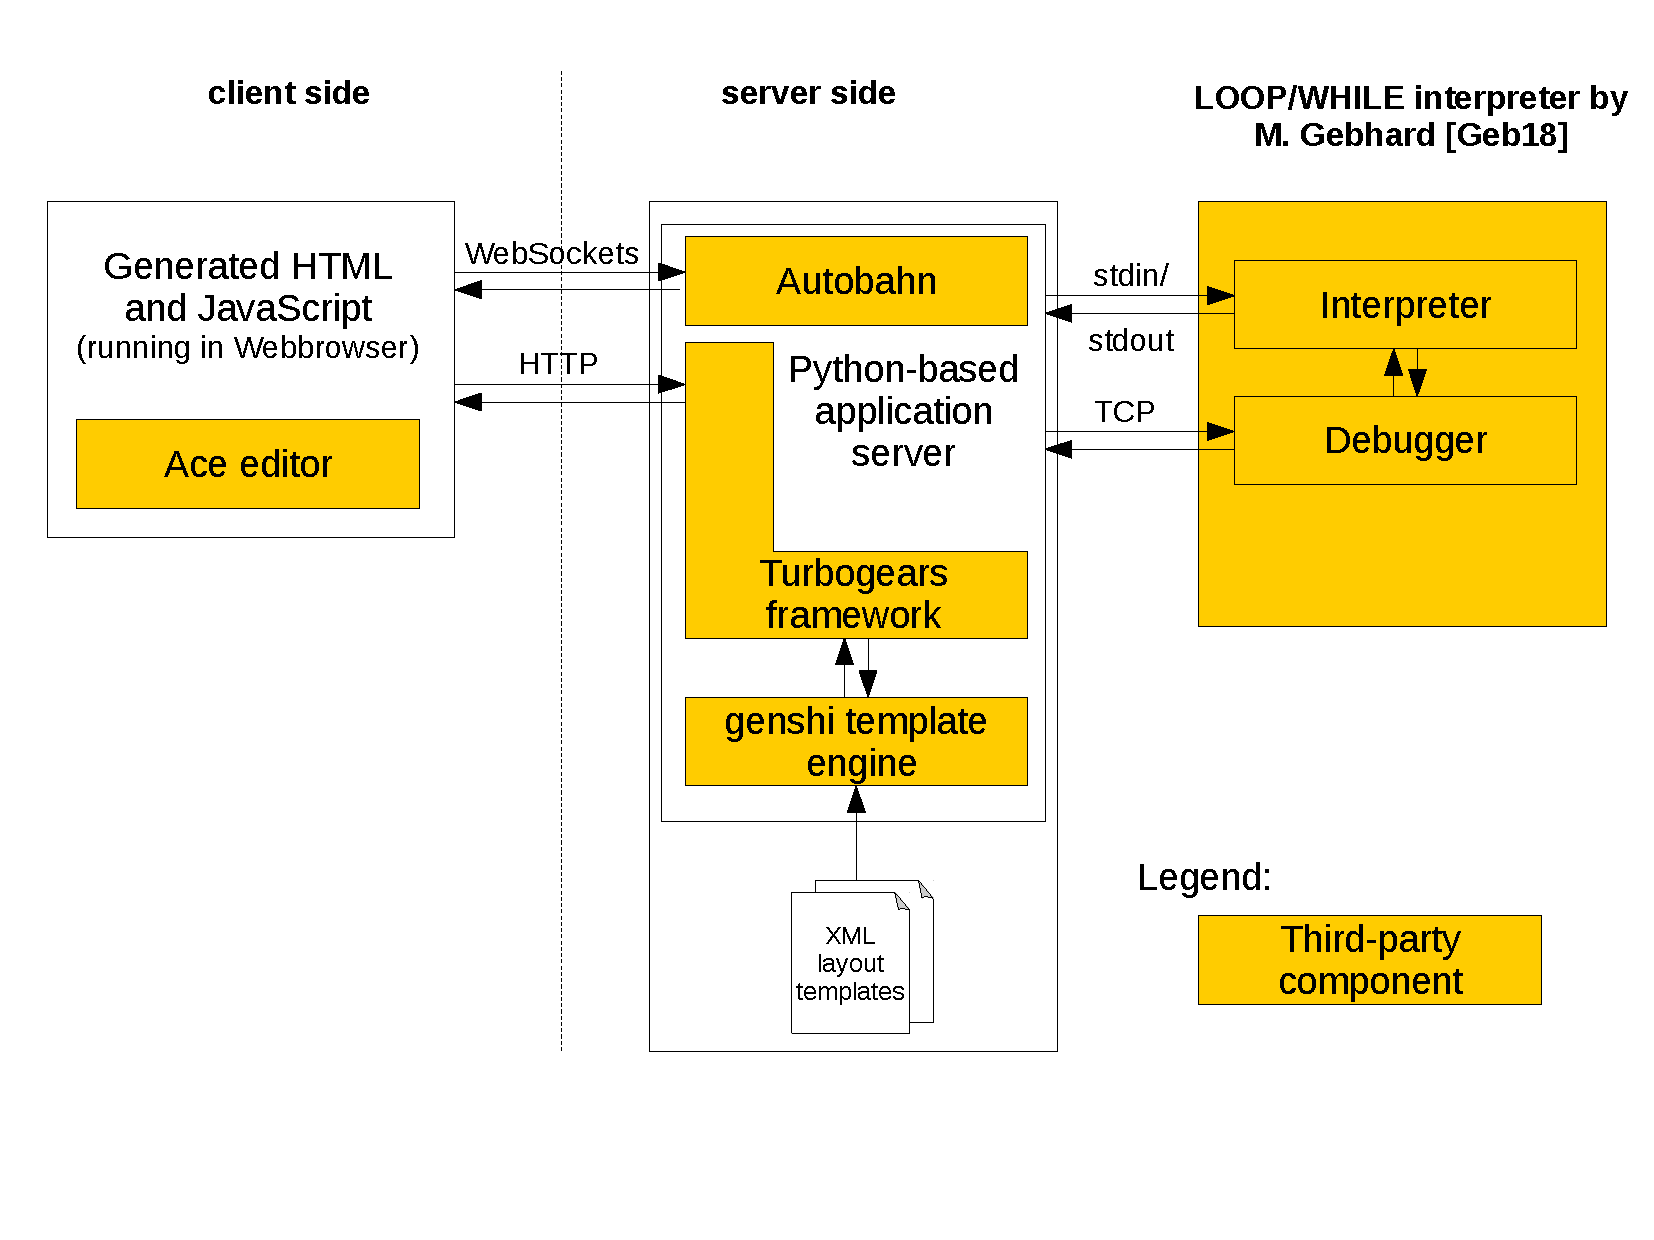
\includegraphics[width=340px]{img/Architecture.pdf}
    \caption[Software architecture]{Software architecture}
    \label{fig:software_arch}
\end{figure}

The view on the client side has two different modes: the interpreter and the debugger mode.
In the interpreter mode, the user sees an editor, realized
by the Ace editor library, in which he can edit his code. When the user clicks the run button, the JavaScript in the browser sends a
request to the server, containing the user's program, and the server replies a randomly generated session id. This session id is then
used by the script for authentication in further requests, e.g. when the contents of the terminal are updated or an user input is transmitted
to the server. On the server side, a child process running the lwre binary is spawned to run the user's Loop/While code. The session (and therefore 
also the child process) is terminated, when either 1) the program terminates itself, 2) the user clicks the stop button or 3) a timeout elapses.

When the user clicks the debug button, the view switches to the debug mode, and the editor is replaced by a HTML-table containing the content of
the editor, with the ability to display breakpoints and highlighting of the currently executed line, as it is needed by the debugger. This view is
generated on the server side and also the child process is spawned when entering the debug mode, since the connection to it is not only necessary
when the program runs, but also to set breakpoints before the execution of the user's code is started.

\section{Communication protocols}
The communication between the client JavaScript and the Python-based server relies on two different OSI Layer 7 protocols.

The first one used for synchronous communication is based on HTTP. It provides several commands to start and stop sessions, transmit user
input in the terminal and to set breakpoints:

\begin{tabular}{l l l}
\hline
relative URL           & POST arguments      & server response\\
\hline
run                    & program\textunderscore code        & \textless SESSION\textunderscore ID\textgreater\space in case of success, 0 in case\\
                       &                                    & of error\\
stop                   & session\textunderscore id          & "OK" in case of success, \textless ERR\textunderscore MSG\textgreater\space in case\\
                       &                                    & of error\\
shell                  & input, session\textunderscore id   & \textless STRING\textgreater\space to print on the terminal\\
check\textunderscore termination\text{*}        & session\textunderscore id          & "running", "terminated", "timeout" or "error"\\
start\textunderscore debug\textunderscore session    & program\textunderscore code        & "OK," + \textless SESSION\textunderscore ID\textgreater\space in case of success,\\
                       &                                    &  "FAIL," + \textless ERR\textunderscore MSG\textgreater\space otherwise\\
debugger               & session\textunderscore id          & an HTML \textless div\textgreater\space -tag containing the\\
                       &                                    & debugger view\\
set\textunderscore breakpoint         & session\textunderscore id, line\textunderscore no & "OK" or "FAIL"\\
remove\textunderscore breakpoint      & session\textunderscore id, line\textunderscore no & "OK" or "FAIL"\\
debugger\textunderscore poll\textunderscore state\text{*}   & session\textunderscore id, line\textunderscore no & "DIED", "RESTARTED", "FAIL" or a JSON-\\
                       &                                    & string containing the last stacktrace\\
debugger\textunderscore action        & session\textunderscore id, action\text{**}     & "OK" or "FAIL"\\
\hline
\end{tabular}

\text{*} deprecated commands that were used before the WebSockets-based protocol was developed.\\
\text{**} the following actions are available:

\begin{tabular}{l l l}
\hline
action      & describtion \\
\hline
start       & starts the debugger and stops at the first line of the root macro\\
continue    & continues the debugger until the next breakpoint is reached.\\
stepinto    & steps to the next line\\
stepover    & steps to the next line without entering macros\\
stepout     & steps out of the current macro\\
close       & stops the debugger and closes the session. The session id gets invalidated\\
\hline
\end{tabular}

For asynchronous communication, another protocol based on HTML5 WebSockets is used.
When a client has started the interpreter or debugger, it connects to the WebSockets
server and transmitts its session id for authentification. By this communication channel,
the client gets notified when the status of the lwre changes, a line can be printed on the
terminal or a debugger breakpoint is reached.

\section{Repository structure}
\begin{tabular}{l l}
\verb|src/|           & source for the backend\\
\verb|templates/|     & XML/XHTML templates for turbogears\\
\verb|web/|           & files that will be directly served by the web server\\
\verb|unit_tests/|    & unit tests for the backend\\
\verb|test_programs/| & test programs that are used by the unit tests\\
\verb|config/|        & sample configuration files\\
\verb|doc/|           & sources of the documentation you are reading
\end{tabular}
